%----------------------------------------------------------------------------------------
%	PACKAGES AND THEMES
%----------------------------------------------------------------------------------------
\PassOptionsToPackage{table}{xcolor}
\documentclass[aspectratio=169,xcolor=dvipsnames,svgnames,x11names,fleqn]{beamer}
% \documentclass[aspectratio=169,xcolor=dvipsnames,fleqn]{beamer}

\usetheme{RedVelvet}

\usefonttheme[onlymath]{serif}



\usepackage{xspace}
\usepackage{amsmath}
\usepackage{amssymb}
\usepackage{amsfonts}
\usepackage{color}
\usepackage{physics}
% \usepackage{mathbb}
\usepackage{rahul_math}
\usepackage{bigints}

\usepackage{graphicx} % Allows including images
\usepackage{booktabs} % Allows the use of \toprule, \midrule and \bottomrule in tables
\usepackage{tikz,pgfplots}
\usepackage{subfigure}
\usetikzlibrary{arrows}
\usepackage{minted}
\definecolor{LightGray}{gray}{0.9}
\definecolor{cream}{rgb}{0.92, 0.9, 0.55}
\definecolor{lightblue}{rgb}{0.68, 0.85, 0.9}


\usepackage{xcolor-material}
\usetikzlibrary{fit}
\tikzset{%
apple/.pic={
  \fill [MaterialBrown] (-1/8,0)  arc (180:120:1 and 3/2) coordinate [pos=3/5] (@)-- ++(1/6,-1/7)  arc (120:180:5/4 and 3/2) -- cycle;
  \fill [MaterialLightGreen500] (0,-9/10)  .. controls ++(180:1/8) and ++(  0:1/4) .. (-1/3,  -1) .. controls ++(180:1/3) and ++(270:1/2) .. (  -1,   0) .. controls ++( 90:1/3) and ++(180:1/3) .. (-1/2, 3/4) .. controls ++(  0:1/8) and ++(135:1/8) .. (   0, 4/7)
}
}

\newcommand{\leftdoublequote}{\textcolor{blue}{\scalebox{3}{``}}}

\newcommand{\rightdoublequote}{\textcolor{blue}{\scalebox{3}{''}}}


\usepackage{textcomp}

\usepackage{overpic}

%----------------------------------------------------------------------------------------
%	TITLE PAGE
%----------------------------------------------------------------------------------------

\usepackage{tikz-qtree,tikz-qtree-compat}
\usetikzlibrary{calc}


\title[CPE 486/586: Machine Learning]{CPE 486/586: Machine Learning for Engineers} % The short title appears at the bottom of every slide, the full title is only on the title page
\subtitle{01 Tools for Machine Learning}

\author[Rahul Bhadani] {{\Large \textbf{Rahul Bhadani}}}

\institute[UAH] % Your institution as it will appear on the bottom of every slide, maybe shorthand to save space
{
    Electrical \& Computer Engineering,  The University of Alabama in Huntsville
}
\date

% \titlegraphic{
%    \includegraphics[width=0.4\linewidth]{figures/UAH_primary.png}
% }

\begin{document}

%-------------------------------------------------
\begin{frame}
  \titlepage
\end{frame}

%-------------------------------------------------
\begin{frame}{Outline}
   \tableofcontents
\end{frame}



\section{Command Line Tools and Linux}

\begin{frame}
    \sectionpage
\end{frame}

\begin{frame}{Why Command Line Tools and Linux}

\begin{enumerate}
    \item Download data from another location, webpage or server \begin{center}
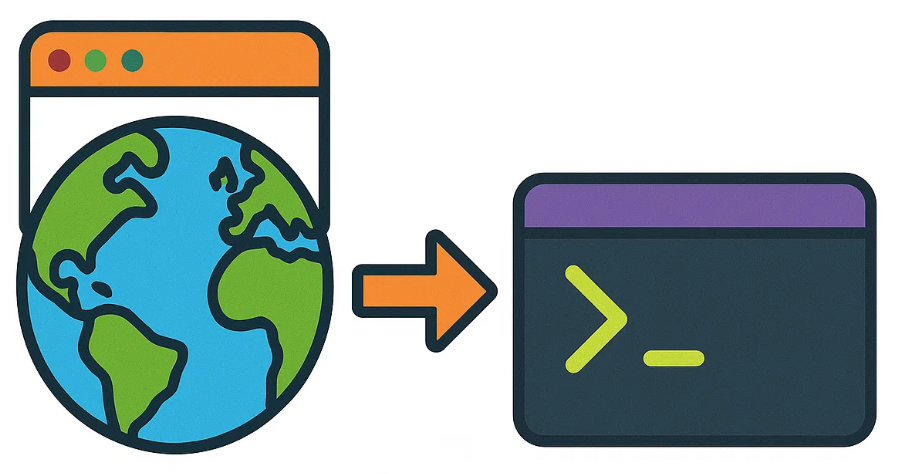
\includegraphics[height=.4\textheight]{figures/cmd_line_download.png}
\end{center}
\end{enumerate}
    
\end{frame}

\begin{frame}{Why Command Line Tools and Linux}

\begin{enumerate}
    \setcounter{enumi}{1}
    \item File operation, renaming, copying, editing, etc, in bulk. 
    \begin{center}
        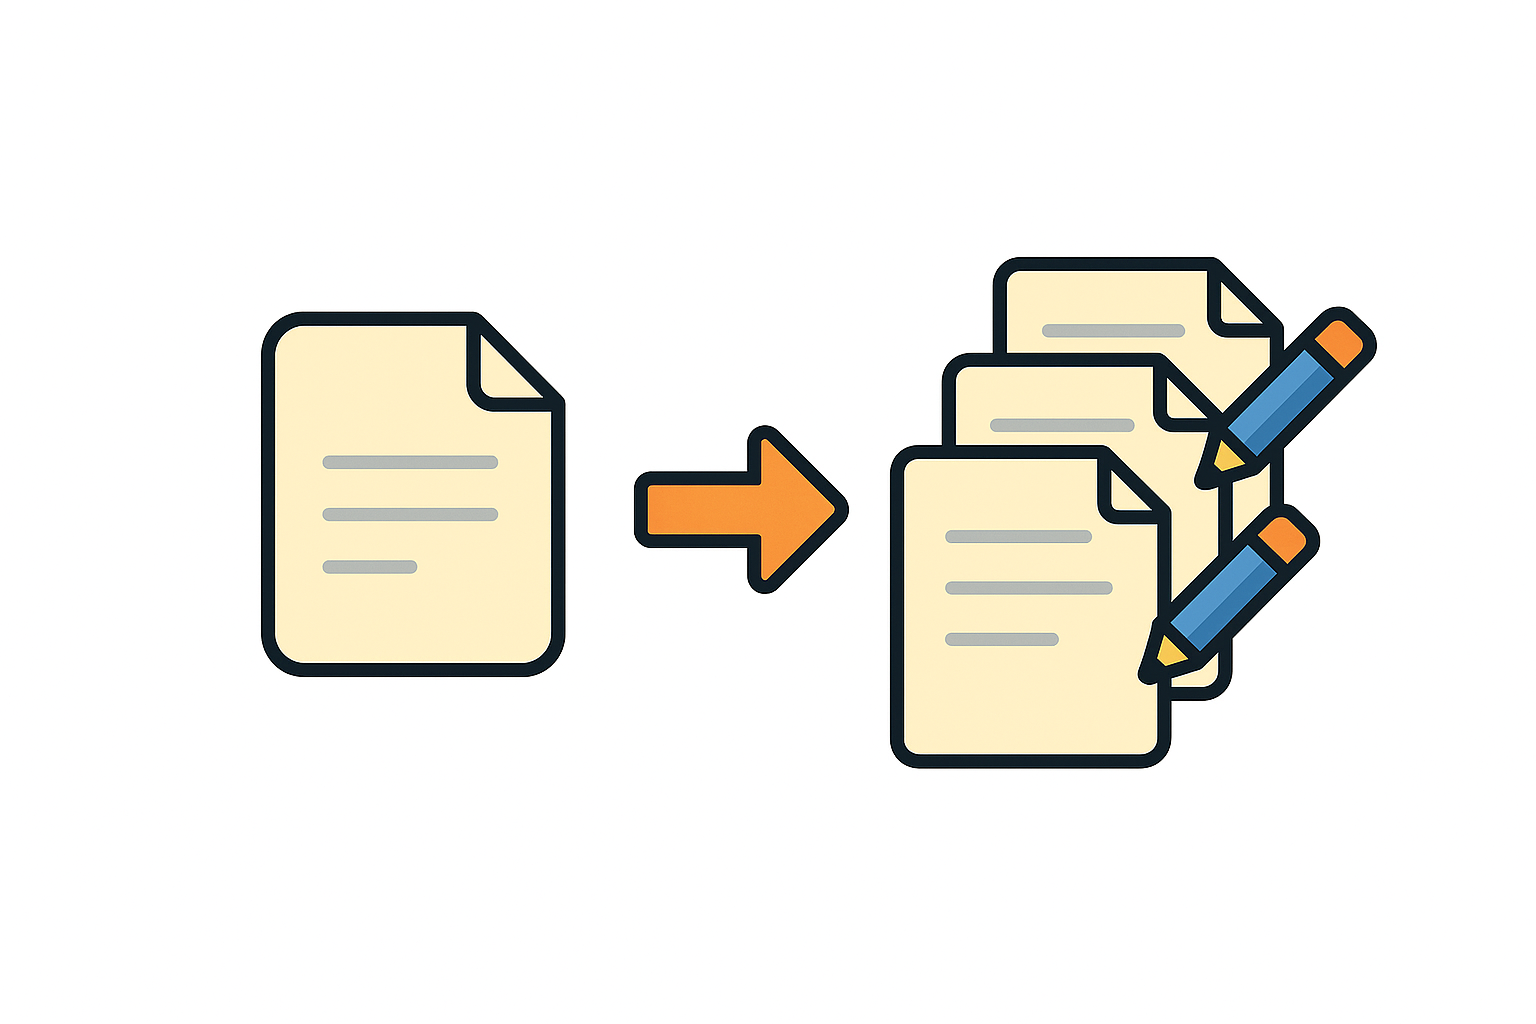
\includegraphics[height=.4\textheight]{figures/FileOperation.png}
    \end{center}

\item Logging into remote server

\item To integrate with other languages and tools.

\item Command Line provides scalability, extensibility, and can automate the entire pipeline for machine learning and data science.


\end{enumerate}
    
\end{frame}

\begin{frame}{Command Line}
    \begin{columns}
        \begin{column}{0.5\textwidth}
            \centering
            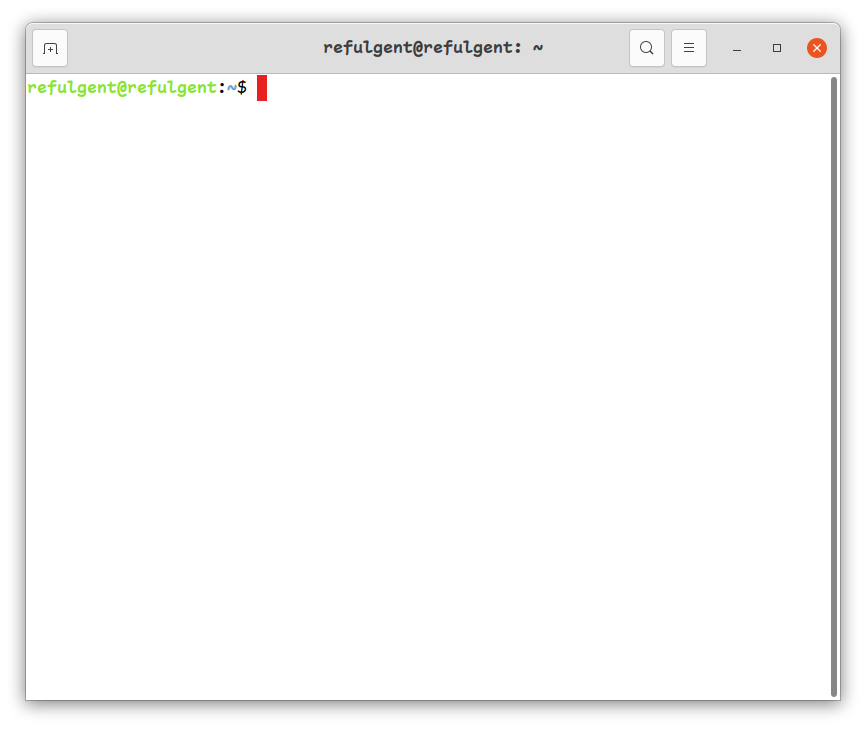
\includegraphics[width=\textwidth,height=1.0\textheight,keepaspectratio]{figures/terminal.png}
        \end{column}
        \begin{column}{0.5\textwidth}
            \begin{enumerate}
                \item Terminals in Linux and Macbook
                \item Windows. Several Options:
                \begin{enumerate}
                    \item Git Bash. Install guide: \url{https://youtu.be/SsdpuprzRE0}
                    \item Cygwin. Install guide: \url{https://youtu.be/_j0Prs7aggo}
                    \item WSL.Install guide: 1. \url{https://youtu.be/GMhV5Uqd8R8},
                    2. \url{https://youtu.be/NPuIUT_6NeM?si=g0N39WfsBf3kIKCx}
                \end{enumerate}
            \end{enumerate}
        \end{column}
    \end{columns}
\end{frame}


\begin{frame}[containsverbatim]{Common Linux Commands}

\footnotesize

My recommendation is to use Windows Subsystem for Linux, as it provides full linux funtionality to Windows.

\vspace{10pt}

A good tutorial to get started is \textbf{Getting started with Linux and Bash
} at \url{https://learn.microsoft.com/en-us/windows/wsl/tutorials/linux}

\begin{tblock}{}

\begin{enumerate}
    \item Installing Software: 
    
    \begin{minted}{bash}
    sudo apt-get install vim git
    \end{minted}

    \item Get the working directory path:
    
    \begin{minted}{bash}
    pwd
    \end{minted}

    \item Change directory:
    
    \begin{minted}{bash}
    cd /data/ch02
    \end{minted}

    \item Create a directory or folder:
    
    \begin{minted}{bash}
    mkdir data
    \end{minted}

\end{enumerate}


\end{tblock}
    
\end{frame}

\begin{frame}
    
    \begin{center}
        An in-depth tutorial is at \url{https://jeroenjanssens.com/dsatcl/chapter-1-introduction}

        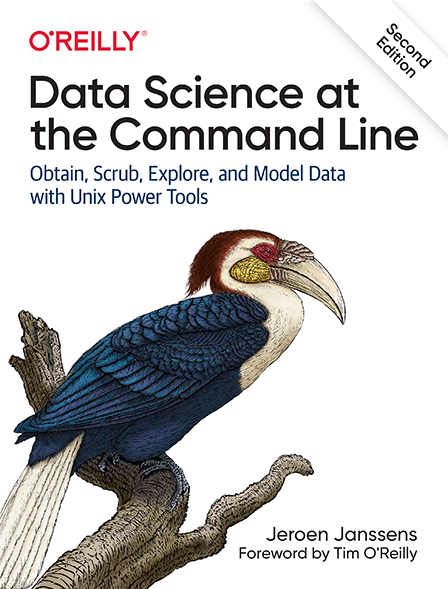
\includegraphics[width=\textwidth,height=0.75\textheight,keepaspectratio]{figures/ds_cmdline.png}

    \end{center}
\end{frame}

\begin{frame}[containsverbatim]{Remote Logging}
    
    If you do not have a powerful machine, you can remotely logging into UAH Engineering Linux Server using your UAH ID.

    \begin{minted}[bgcolor=powderGreen]{bash}
    ssh rkb0022@blackhawk.ece.uah.edu
    \end{minted}

    Windows users should use WSL Terminals.

\end{frame}



\section{Python}

\begin{frame}
    \sectionpage
\end{frame}


\begin{frame}[containsverbatim]{Installing Python}
    
    Most machine learning libraries and codebase are written Python. Python is supported by a strong open-source community.

    Windows users download from \url{https://www.python.org/downloads/}

    Mac users download from \url{https://www.python.org/downloads/macos/}

    Linux users install from command line

    \begin{minted}[bgcolor=powderGreen]{bash}
    sudo apt-get install python3.12
    \end{minted}

    or 

    \begin{minted}[bgcolor=powderGreen]{bash}
    sudo apt-get install python3.12-full
    \end{minted}

    Recommended version of Python for this course is Python 3.12.

\end{frame}

\section{Git and GitHub}

\begin{frame}
    \sectionpage
\end{frame}

\begin{frame}[containsverbatim]{Version Controlling your Development}
    It is must that any of your machine learning project, and in general any coding project should use Git.

    You should already have Git installed in your system through Git, otherwise install.

    \begin{enumerate}
        \item Create a GitHub account and a user name.
        \item Create a new repository.
        \item Clone to local machine:
        
        \begin{minted}[bgcolor=powderGreen]{bash}
        git clone https://github.com/rahulbhadani/TestRepo TestRep
        \end{minted}

    \end{enumerate}
\end{frame}

\begin{frame}[containsverbatim, allowframebreaks]{Commonly used Git Commands}

    \footnotesize

    \begin{enumerate}
        \item Initialize an existing local folder as a git repo.
        \begin{minted}[bgcolor=powderGreen]{bash}
        git init
        \end{minted}
        \item Add remote to your local git folder (Only needs to do once per repo).
        \begin{minted}[bgcolor=powderGreen]{bash}
        git remote add origin https://github.com/rahulbhadani/TestRepo.git
        \end{minted}
        \item Add files for commit.
        \begin{minted}[bgcolor=powderGreen]{bash}
        git add . # add all files
        git add somefile.txt # Add specific file(s)
        \end{minted}
        \item Commit changes with a message before you push to the remote.
        \begin{minted}[bgcolor=powderGreen]{bash}
        git commit -m "Added some files" # add a meaninful message
        \end{minted}
        \item Push to the remote.
        \begin{minted}[bgcolor=powderGreen]{bash}
        git push  # shortcut command
        git push -u origin # push to a specific remote named origin
        git push -u origin2 HEAD:master # push to specific origin's specific branch
        \end{minted}
        \item Pull updates from a remote.
        \begin{minted}[bgcolor=powderGreen]{bash}
        git pull  # shortcut command
        git pull origin master # pull from specific remote
        \end{minted}

        \item Git undo add before commit
        \begin{minted}[bgcolor=powderGreen]{bash}
        git reset filename.txt
        \end{minted}
        \item Git undo add after commit but before push and keep your changes
        \item \begin{minted}[bgcolor=powderGreen]{bash}
        git reset --soft HEAD~1
        \end{minted}
        \item Git undo add after commit but before push and unstage
        \item \begin{minted}[bgcolor=powderGreen]{bash}
        git reset HEAD~1
        \end{minted}
        \item Git undo add after commit but before push and discard every changes
        \item \begin{minted}[bgcolor=powderGreen]{bash}
        git reset --hard HEAD~1 # use n for undoing n multiple commits
        \end{minted}
    \end{enumerate}
    
\end{frame}

\section{Development Environment}

\begin{frame}
    \sectionpage
\end{frame}

\begin{frame}{Integrated Development Environment (IDE)}

    Why use IDEs?
    \begin{enumerate}
        \item Provides integrated view of editor, file explorer, command lines.
        \item Some IDEs provide intellisense for autocomplete.
        \item IDEs are also integrate with compiler/inteprerter -- one click to run your code.
        \item IDEs are beautiful, rich colors and fonts over boring plain text editors.
        \item Many IDEs add support for additional features such as visualization, remote log in, data wranling, etc.
    \end{enumerate}
    
\end{frame}

\begin{frame}{VS Code}
    
    Many IDEs are available such PyCharm, Atom, VS Code.

    \vspace{10pt}

    For this course, I recommend VS Code.

    \begin{center}
        
\includegraphics[width=\textwidth,height=0.45\textheight,keepaspectratio]{figures/vscode.png}
    \end{center}

    VS Code supports several extensions for Python, and other necessary tools.

\end{frame}






\section{Packages and Package Manager}

\begin{frame}
    \sectionpage
\end{frame}


\section{Jupyter Notebook}

\begin{frame}
    \sectionpage
\end{frame}


\section{Markdown}

\begin{frame}
    \sectionpage
\end{frame}

\section{Latex}

\begin{frame}
    \sectionpage
\end{frame}

\section{Other Notable Tools}

\begin{frame}
    \sectionpage
\end{frame}

\begin{frame}
    \Huge{\centerline{\color{bubblegumPink}\textbf{The End}}}
\end{frame}



\end{document}